\chapter{Úvod}

	Dnes lze najít spoustu řešení pro řízení doma postaveného CNC stroje. Většina z~nich je postavena na~osobním počítači, který vykonává veškeré nutné úkony – od zpracování vstupního G-kódu, přes výpočet rychlosti a generování řídicích signálů pro pohony, až po samotné uživatelské rozhraní. Tento koncept je velmi jednoduchý na~realizaci (počítač poskytuje dostatek výpočetního výkonu a přívětivé rozhraní pro uživatele), zároveň je také velice levný – není třeba žádné speciální vybavení.
	
	To s sebou přináší však i~řadu nevýhod. Mezi největší řadím omezené možnosti generování výstupního řídicího signálu (zejména co se výstupní frekvence a doby odezvy týče). Klasický stolní počítač disponuje mnohonásobně větším výkonem než jednočipové mikrokontroléry, avšak narozdíl od jednočipu mu jeho koncepce neumožňuje provádět přesné výstupní operace, co se časování týče.
	
	Také tyto systému často disponují nepropracovaným systémem řízení rychlosti, který většinou spoléhá na~kvalitní a tuhou konstrukci stroje, která je často u~hobby strojů právě nejslabším článkem.
	
	\section{Cíle projektu}	
	Výše uvedené důvody mě motivovaly k~tomu pokusit se navrhnout a~posléze i~realizovat vlastní řídicí systém, který by tyto nedostatky měl odstranit. Můj systém by měl řídit tříosou frézku v~klasickém pravoúhlém uspořádání, což je nejčastější a~nejjednodušší možné uspořádání. Vstupní data by měl přebírat v~G-kódu, který je nepsaným standardem pro programování CNC strojů, a~měl by také podporovat funkce pro kompenzaci nástroje.

\chapter{Koncepce řídicího systému hobby CNC stroje}

	V~domácích podmínkách není možné dosáhnout na~prostředky běžně používané v~průmyslovém prostředí. Roli zde hrají nejen finance, ale také výrobní možnosti. Na hobby CNC stroj však nejsou kladeny takové nároky jako na~průmyslové stroje. Proto se často přistupuje k~jednodušším řešením, která však pro nenáročné hobby použití dostačují..
	
	Na schématu \ref{nak:hobby} znázorňuji běžné uspořádání řídicího systému hobby CNC strojů. Toto schéma jsem sestavil na~základě strojů ze sekce \uv{Naše mašinky} na~diskusním fóru C-N-C.cz \cite{c-n-c}.
	
	\begin{figure}[h]
		\centering
		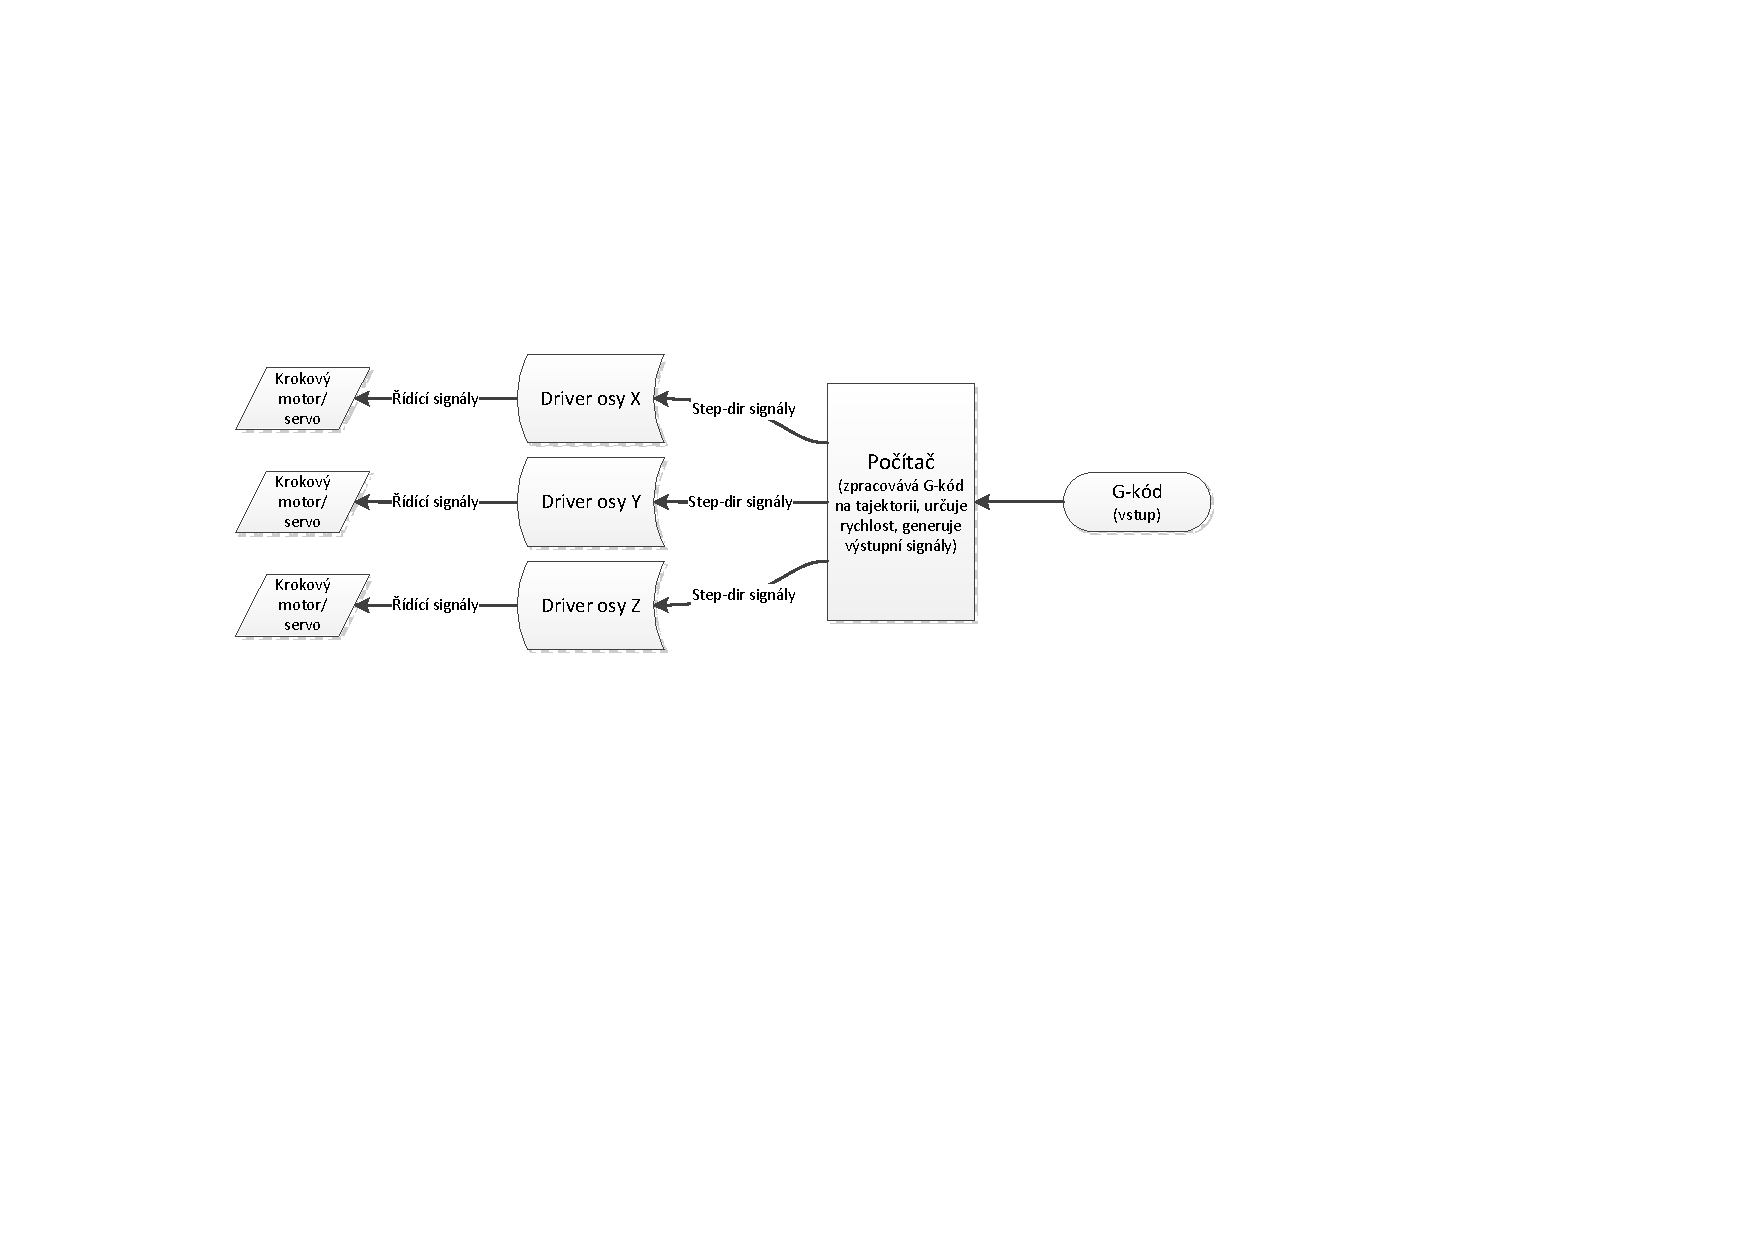
\includegraphics[width=0.9\textwidth]{img/HobbyCNC.pdf}
		\caption{Schéma znázorňující uspořádání klasického řídicího systému hobby CNC stroje.}\label{nak:hobby}	
	\end{figure}
	
	\section{Pohony}
	Pro řízení hobby CNC strojů se používají krokové motory, zřídka servomotory. Zpravidla se nepoužívá žádná zpětná vazba do řídicí jednotky (i zpětná vazba z~enkodérů u servomotorů je zpracovávána pouze v rámci pohonu). Na řízení krokových motorů a~servomotorů se používají speciální drivery, které příjmají informaci ve formátu step-dir. Úroveň jednoho datového vodiče určuje směr otáčení, vstupní pulz na~druhém pak \uv{krok} -- pootočení motoru o daný úhel. Při řízení se spoléhá na~to, že pohon je dostatečně nadimenzovaný a~nedojde ke~ztrátě kroků.
	
	\paragraph{Krokové motory} jsou velmi levnou variantou pohonu. Jejich výhodou je jednoduchý způsob řízení a~velký přídržný moment. Pro jejich řízení existují i~speciální itegrované obvody -- např.~hojně používané Toshiba TB6560\cite{TB6560}. Nevýhodou krokových motorů je jejich malý moment ve vysokých otáčkách a~relativně \uv{tvrdý chod} (motor se pohybuje po přesně daných krocích) -- vznikají rezonance\cite{krokovymotor}.
	
	\paragraph{Servomotory} v~poloprofesionálním provedení se skládají ze~stejnosměrného či bezkomutátorového motoru, ke kterému je připevněn rotační encoder\cite{servomotor}. Na základě požadované pozice a~reálné pozice motoru získané z~enkodéru se tvoří řídicí signál pro motor. Ačkoliv zde již zpětná vazba existuje, není posílána zpět do systému. Servomotory mají oproti krokovým motorům také lepší moment při vyšších otáčkách\cite{servomotor}. Avšak používaný systém řízení step-dir trochu degraduje jejich možnosti (při nízkém počtu kroků na~otáčku je nutí pracovat v~nespojitém režimu).
	
	\section{Generování řídicích signálů}
	Řídicí signály zpravidla generuje počítač pomocí pinů paralelního portu. Pro správnou funkci je třeba generovat pulzy v~řádech stovek Hz až jednotek kHz. Zde spatřuji největší slabinu těchto řídicích systémů. Klasický počítač není stavěn na~přesné generování výstupních signálů v~\uv{režimu GP~I/O}. Částečně je možné přesné časování zajistit použitím real-timového operačního systému, avšak i~přesto nelze dosahovat závratných výsledků.
	
	Řešením může být použití interpolátoru postaveného na~mikrokontroléru, kde není problém generovat přesně dané pulzy v~přesně daném časovém rámci (až s~přesností na~nanosekundy), či použít speciální přídavné karty do PCI, popř. PCIe, slotu, která přidá do počítače podporu pro GP~I/O.
	
	\section{G-kód}
	G-kód je označení jazyka pro zápis drah CNC stroje\cite{wiki:gcode}. Tento jazyk se používá jak v~průmyslovém prostředí, tak i~v~hobby. Dráhy stroje lze programovat ručně, dnes se však již i~mezi hobby uživateli používá CAM program, který G-kód vygeneruje (téměř) automaticky. Standard tohoto jazyka však není většinou respektován a~každý systém některé jeho části interpretuje různě.
	
	V~základu disponuje G-kód prostředky pro zapsání lineární a~obloukové interpolace\cite{gcode}. Objevily se však snahy zaimplementovat podporu pro obecné křivky (např. systém Sinumerik 810~T implementuje podporu pro spline\cite{sinumerik}). Avšak tato řešení se neujala v~praxi. Osobně se domnívám, že je to zapříčiněno nulovou podporou v~CAM programech. Složitější křivky se tedy i~dnes zapisují jako řada na~sebe tečných kruhových oblouků, které danou křivku pouze aproximují.
		
	\section{Existující řešení řídicího sytému}

	Na závěr této kapitoly jsem zařadil stručný přehled již existujících řídicích systémů, které jsou běžně používány. 
	
		\subsection{Mach 3}
		
		Mach 3 je řídicí systém od společnosti ArtSoft\cite{mach3}. Tento software je určen pro stolní počítače s~operačním systémem Windows. Je cílen na~amatérské až poloprofesionální použití a~je schopen ovládat až 6~os. Mach 3 využívá lineárních akceleračních křivek -- používá konstantní zrychlení a~nijak nelimituje ryv\cite{mach3}. Podporuje pouze stroje s pravoúhlým uspořádáním os.
		V~základní verzi je dostupný zdarma, avšak omezuje maximální délku načítaného programu.
		
		Veškeré vstupně-výstupní operace probíhají přes piny paralelního portu. Avšak díky absenci real-time kernelu ve~Windows není schopen generovat vysoké řídicí frekvence. To potvrzují zkušenosti uživatelů z~diskusního fóra C-N-C.cz\cite{c-n-c}. Vesměs označují systém za nestabilní a~fungující pouze na~konkrétním hardwaru. Avšak lze najít spoustu spokojených uživatelů tohoto systému – většinou se však nesnaží dosáhnout vysokých obráběcích rychlostí.
		
		Zajímavou vlastností Machu 3 je existence relativně velkého počtu různých tzv. hardwarových stepgenů\footnote{Přehled všech dostupných řešení lze nalézt na~\url{http://www.machsupport.com/plugins.php}}. Stepgeny jsou diskrétní kousky hardwaru postaveného na~mikrokontroléru či FPGA, které se připojují k~počítači pomocí komunikačního rozhraní (USB, paralelní či sériový port). Ze systému dostávají instrukce o aktuálním pohybu a~až stepgen generuje řídicí signály pro pohony stroje. Tím je odstraněn problém přesného časování výstupních operací. V podstatě se jedná o stejnou formu řešení jako můj řídicí systém. Příkladem stepgenu může být SmoothStepper\footnote{\url{http://www.warp9td.com/}}. Tyto stepgeny však nejsou příliš rozšířeny a~nepovedlo se mi zjistit žádné uživatelské zkušenosti.
		
		\subsection{Linux CNC}
		
		LinuxCNC, dříve nazývaný EMC (Endhanced Machine Controller), je open source projekt univerzálního řídicího systému postaveného na~stolním počítači\cite{linuxcnc}. Narozdíl od Machu 3 běží LinuxCNC pod Linuxem s~kernelem obohaceným o RT API (real-time API), které umožňuje spouštět určité operace v přesně daném čase (přesnost je omezena použitým hardwarem počítače).
		
		LinuxCNC staví na~univerzálnosti. Je plně konfigurovatelný a~přizpůsobitelný. Osobně se mi na~něm líbí koncept HAL (hardware abstraction layer)\footnote{Podrobnosti o systému lze najít v manuálu: \url{http://www.linuxcnc.org/docs/HAL\_User\_Manual.pdf}}, který umožňuje zcela libovolně propojit vstupy a~výstupy jednotlivých komponent nejen s~hardwarovým výstupem, ale i~mezi sebou. Systém je téměř libovolně upravitelný. Díky tomu je však komplikovaný, což může odradit spoustu uživatelů. 
		
		Z hlediska dynamiky používá LinuxCNC také lineární akcelerační křivku. Systém však zvládá výpočet rychlosti pro několik druhů kinematiky stroje -- nejen pravoúhlé, ale např. i~tzv. hexapodu.
		
		Vstupně-výstupní operace jsou realizovány za pomoci paralelního portu. Avšak díky RT kernelu dosahuje vyšší spolehlivosti (dle zkušeností uživatelů C-N-C.cz fóra\cite{c-n-c}). Je méně závislý na~použitém hardwaru počítače, avšak i~přesto existují konfigurace, na~kterých neběží spolehlivě.
		
		Pro tento systém existuje podpora MESA karet\footnote{\url{http://www.mesanet.com/}}. Jedná se o karty, nejčastěji do PCI či PCIe slotu, osazené FPGA, na~kterých je přenecháno generování výstupních signálů. Při použití těchto karet dosahuje systém vyšší spolehlivosti, avšak stále není možné vypustit real-time kernel.
		
		\subsection{Intepolační jednotky Gravos}
		
		Česká společnost Gravos vyvíjí a~vyrábí vlastní řídicí systém, resp. celý balík CAD, CAM programu a~řídicího systému\cite{gravos}. Tento systém využívá nezávislou řídicí jednotku postavenou na~ARM mikrokontroléru. Tato jednotka s~počítačem komunikuje pomocí sériového portu, z~nějž získává data a~realizuje uživatelský vstup a~výstup.
		
		Koncepcí se mi tento systém líbí a~na základě něj jsem se i~trochu inspiroval pro koncepci mého řídicího systému. Řídící jednotka generuje step-dir signály. Nikde na~stránkách společnosti jsem však nenašel informace o použité akcelerační křivce. Rozhodl jsem se proto společnost kontaktovat se žádostí o~podrobnější informace. Obdržel jsem velmi vstřícnou odpověď (kopie odpovědi se nachází v~příloze \ref{kap:gravos}).
		
		Pro obrábění se používají lineární akcelerační křivky, avšak pro rychloposuv je implementována i~S-křivka. Na tomto systému mě překvapilo, jak elegantně byl vyřešen problém s~dynamikou stroje pohybu po kruhovém oblouku. Do systému se zadávají dvě omezení maximálního zrychlení -- jedno pro pohyb po přímce, druhé pro pohyb na~oblouku o poloměru 1~mm, z~nějž lze dopočítat zrychlení pro oblouk o libovolném poloměru. Ačkoliv se nejedná o fyzikálně podložené řešení, tak po experimentálním zjištění vhodného limitního zrychlení musí v~praxi fungovat nadmíru dobře.
		
		Zajímavý je také přístup k~interpolaci kruhového oblouku. Veškeré křivky jsou rozloženy na~sérii přímých úseků. Pokud se nastaví délka těchto úseků blízko, či dokonce pod rozlišovací schopnost pohonů, může systém naprosto přesně projet libovolnou křivku při zachování jednoduchosti interpolační jednotky.
		
\chapter{Koncepce mého řídicího systému}

	Koncepci mého řídicího systému znázorňuje schéma \ref{nak:muj}. Řídicí systém se skládá ze dvou částí -- počítače zajišťujícího uživatelský vstup, zpracování G-kódu na~interní formát a~výpočet mezních rychlostí. Druhou částí systému je nezávislý interpolátor, který přebírá již zpracované informace o jednotlivých úsecích a~na základě nich generuje řídicí step-dir signály (provádí tedy samotnou interpolaci).

	\begin{figure}[h]
		\centering
		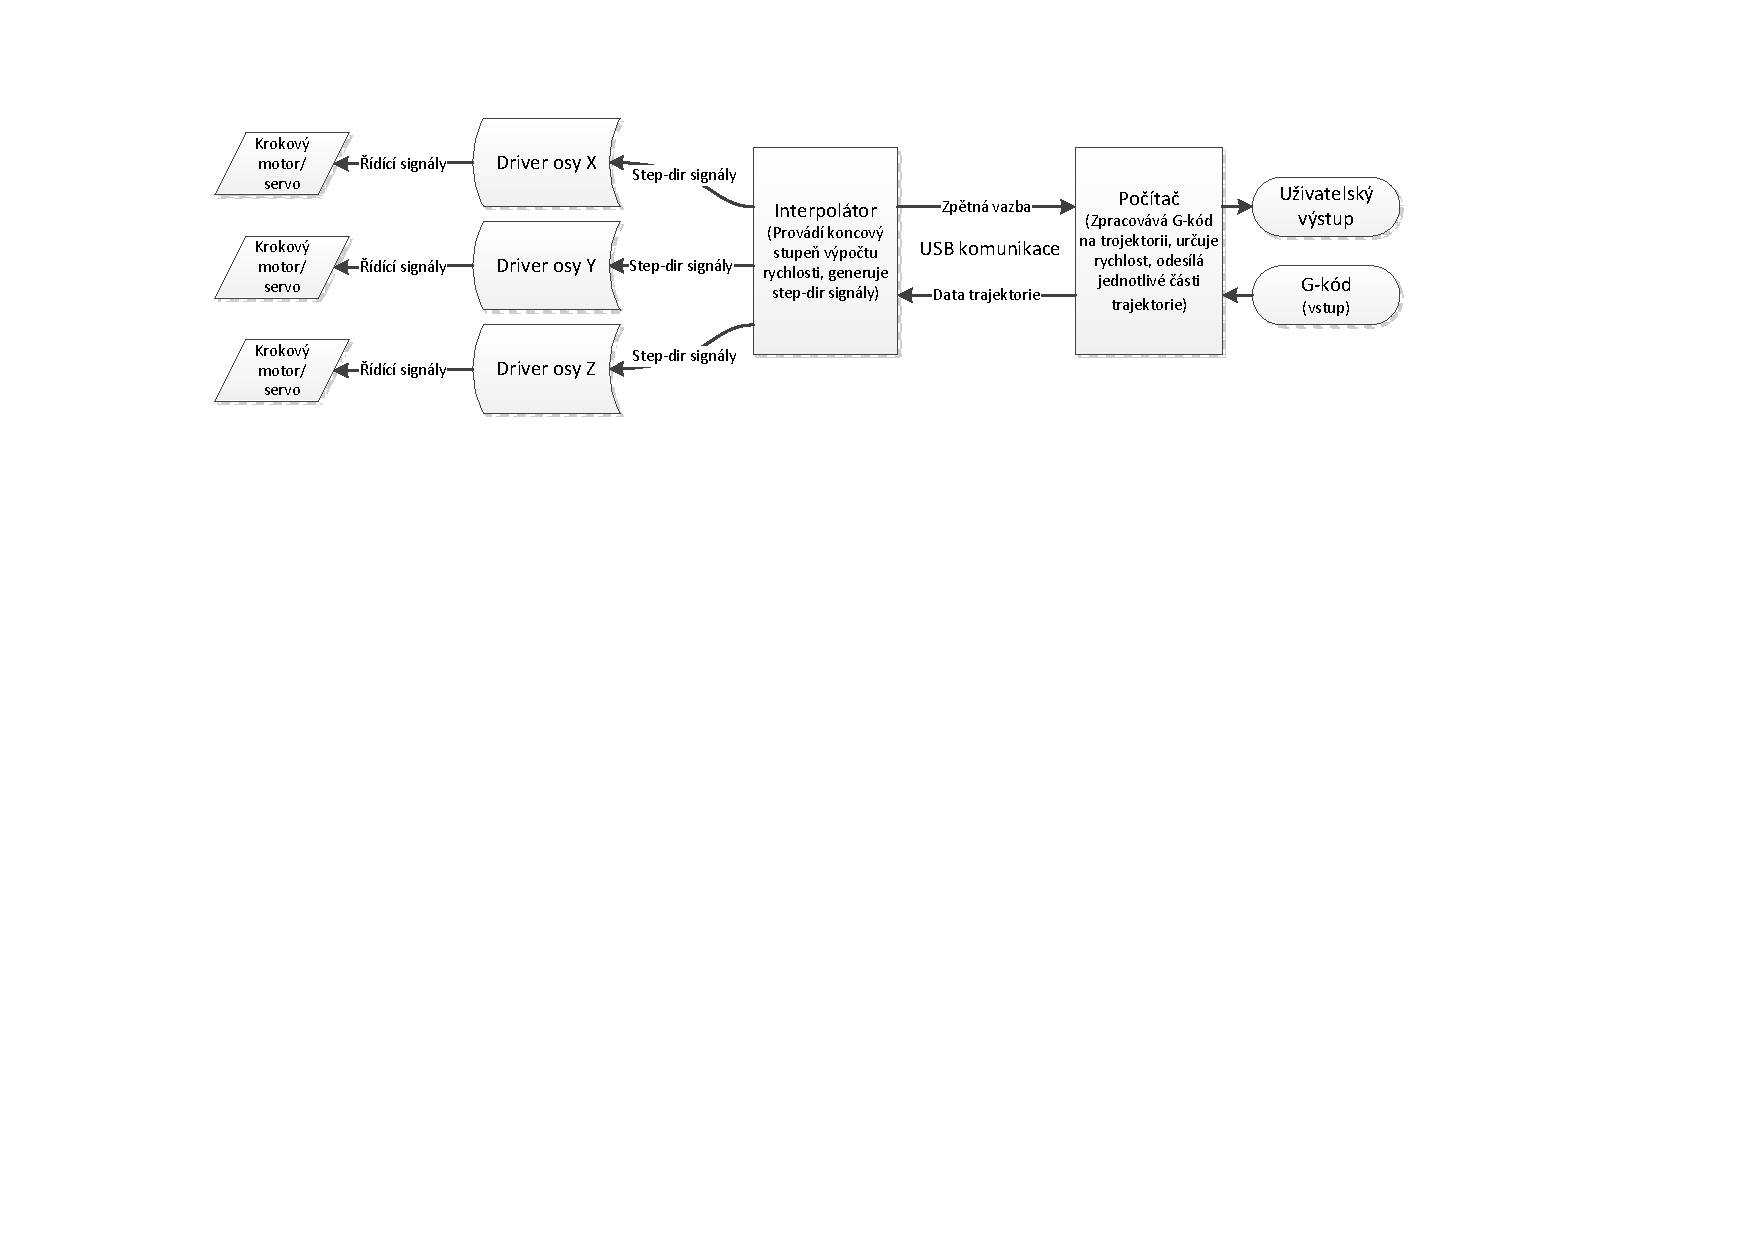
\includegraphics[width=1\textwidth]{img/mujsystem.pdf}
		\caption{Schéma znázorňující uspořádání mého řídicího systému.}\label{nak:muj}	
	\end{figure}
	
	Použítí interpolátoru postaveného na~jednočipovém mikrokontroléru byla jasná volba -- pouze tak lze docílit kvalitního výstupního signálu a~spolehlivosti stroje. Na jednočipu je totiž možné narozdíl od počítače uhlídat přesné časování a~generovat vyšší výstupní frekvence.
	
	Jako komunikační rozhraní mezi počítačem a~interpolátorem jsem zvolil USB, ani ne tak díky jeho rychlosti (nepřenáší se velká kvanta dat), ale díky jeho jednoduchosti, co se uživatele týče. Narozdíl od sériové linky nemusí uživatel vybírat správný port a~má aplikace je schopna detekovat správné připojení zařízení. Navíc při použití integrované USB periférie v~mikrokontroléru můžu na~komunikaci pohlížet jako na~\uv{black box} a~nemusím se starat o integritu dat -- data dostanu vždy správně napaketovaná tak, jak jsem je odeslal.
	
	Narozdíl od řídicího systému Gravos by měl můj interpolátor umět generovat řídicí signály jak pro lineární, tak i~pro obloukovou interpolaci. Z počítače jednotka obdrží pouze informace o typu úseku, jeho charakteristice (počáteční a~koncový bod) a~daných omezeních (počáteční a~koncová rychlost, či maximální zrychlení).
	
	Z výše uvedeného by se mohlo zdát, že role počítače je zde zbytečná -- jednotka skoro vše obstarává sama. Počítač je zde zařazen hlavně kvůli komunikaci s~uživatelem a~jednoduchosti vývoje. Vyvinout uživatelské rozhraní pro počítač je mnohem jednodušší než se snažit připojit display k~mikrokontroléru a~vyvíjet od nuly. Navíc uživatelské rozhraní pro počítač může být mnohem sofistikovanější (vzniká zde komfort při práci se soubory, či je velmi jednoduché provádět změny programu přímo u~stroje).
	
	Počítač zde navíc slouží jako výkonná výpočetní jednotka se spoustou paměti. Jelikož se chci přiblížit co nejideálnějšímu pohybu, je pro určení některých limitů třeba relativně složitých výpočtů. Díky počítači si můžu dovolit takový komfort, jako připravit si celou trajektorii stroje dopředu ještě před tím, než začne samotný pohyb stroje, a~tak vyřešit všechny případné řetězové závislosti.
	
	V následující části \nameref{part:model} (\ref{part:model}) řeším teorii co nejideálnějšího pohybu a~odvozuji vlastní fyzikální model pohybu. V~části \nameref{part:realizace} (\ref{part:realizace}) se zaměřuji na~implementaci odvozeného fyzikálního modelu, popisuji použitý hardware a~návrh programu jak na~straně počítače, tak i~na straně interpolátoru.
	
	